\documentclass{beamer}

\usetheme{Warsaw}
\usecolortheme{seahorse}
\setbeamertemplate{navigation symbols}{}
\setbeamercolor{background canvas}{bg=}
\usepackage{beamerthemesplit}
\usepackage{pgf}
\usepackage{epsfig}
\usepackage{epstopdf}
\usepackage{graphicx}
\usepackage{slashbox}
\usepackage{url}
\usepackage{listings}
\usepackage{polski}
\usepackage[utf8]{inputenc}
\newcommand{\IR}{\bbold R}
\def\Rset{\mathbb{R}}
\def\Zset{\mathbb{Z}}
\newcommand{\refbr}[1]{(\ref{#1})}
\newcommand{\beq}{\begin{equation}}
\newcommand{\eeq}{\end{equation}}
\newcommand{\und}[1]{\underline{#1}}
\newcommand\pro{\item[$+$]}
\newcommand\con{\item[$-$]}
\newcounter{saveenumi}
\newcommand{\seti}{\setcounter{saveenumi}{\value{enumi}}}
\newcommand{\conti}{\setcounter{enumi}{\value{saveenumi}}}

\hypersetup{
   pdftitle={Oprogramowanie do gier opartych o planszę w postaci szachownicy},
   pdfauthor={Jakub Ostrzołek},
   pdfborder={0 0 0}
}

\title[Silnik gier opartych o szachownicę \insertframenumber/\inserttotalframenumber]{
   Projekt i wykonanie oprogramowania do gier planszowych opartych
   o planszę postaci szachownicy – podejście w oparciu o dedykowany
   język dziedzinowy.}
\author[Jakub Ostrzołek]{\textbf{Jakub Ostrzołek \\%
\footnotesize Promotor: dr inż. Patryk Chaber}}
\institute{Instytut Automatyki i Technik Informacyjnych\\%
Politechnika Warszawska}

\begin{document}

\frame{\titlepage}

\frame{\tableofcontents\frametitle{Plan prezentacji}}

\section{Cel pracy}
\begin{frame}
   \frametitle{Cel pracy}
   2 główne cele pracy:
   \begin{enumerate}
      \item opracowanie formatu pliku do opisywania zasad gier planszowych opartych o szachownicę
      \item implementacja interpretera ww. formatu (silnika gry)
   \end{enumerate}
\end{frame}

\section{Tematyka pracy}

\begin{frame}
   \frametitle{}
   \begin{itemize}
      \item plansza 
   \end{itemize}
\end{frame}

\begin{frame}
   \frametitle{Format zasad - wstępne założenia}
   \begin{itemize}
      \item Format pliku zasad jest kluczowym elementem rozwiązania
      \item Wstępne założenia:
            \begin{itemize}
               \item pozwala wyrazić zasady min. rodzajów 3 gier
               \item możliwie nieskomplikowany
               \item zwięzły
               \item wymaga rozumienia podstawowych zasad programowania
            \end{itemize}
   \end{itemize}
\end{frame}

\begin{frame}
   \frametitle{Format zasad - podejścia}
   Możliwe podejścia:
   \begin{enumerate}
      \item Użycie istniejącego formatu (np. {\tt JSON}, {\tt YAML})
            \begin{itemize}
               \pro popularne formaty danych
               \pro brak potrzeby tworzenia parsera
               \con brak łatwego zapisu wyrażeń, funkcji, pętli, itp.
            \end{itemize}
      \item Stworzenie DSL zanurzonego w języku programowania (np. Kotlin, Haskell, Lua)
            \begin{itemize}
               \pro dostępne wszystkie możliwości języka nadrzędnego
               \pro znajoma składnia dla użytkowników
               \con trudno ograniczalny (problem bezpieczeństwa)
            \end{itemize}
      \seti
   \end{enumerate}
\end{frame}

\begin{frame}
   \frametitle{Format zasad - podejścia cd.}
   \begin{enumerate}
      \conti
      \item Stworzenie własnego języka DSL od zera
            \begin{itemize}
               \pro całkowita możliwość dostosowania języka do potrzeb
               \con tworzenie parsera bardzo pracochłonne
               \con brak dodatkowych narzędzi (formatter, linter, itp.)
               \con brak znajomości języka u użytkowników
            \end{itemize}
   \end{enumerate}
\end{frame}

\begin{frame}
   \frametitle{Format zasad - wybór podejścia}
   Wybrałem podejście 1, jednak z niestandardowym formatem - HCL
   \begin{itemize}
      \item sprawdzony format używany m. in. w Terraformie
      \item zawiera elementy standardowych języków programowania:
      \begin{itemize}
         \item ewaluacja wyrażeń arytmetycznych i logicznych
         \item wykonywanie predefiniowanych funkcji
         \item pętle w postaci list/dictionary comprehensions
      \end{itemize}
      \item oficjalny dodatek {\tt userfunc} z funkcjami użytkownika
   \end{itemize}
\end{frame}

\section{Istniejące rozwiązania}

\begin{frame}
   \frametitle{BGD - BoardGameDescription}

   \begin{itemize}
      \item ogólny język opisu gier planszowych
   \end{itemize}

\end{frame}

\begin{frame}[fragile]
   \section{Zadania pracy}
   \frametitle{The installation and starting jPar}
   It is very simple:
   \begin{enumerate}
      \item Copy file .java.policy to home directory (in Windows use
            " Documents and Settings$\setminus$Username" directory) or use "install.bat" (Windows)
            or "sh ./install.sh" (Unix) on every node, where you want to run
            jPar client or solver
      \item Run one instance of paralize server using "jpar\_server.bat" (Windows)
            or "sh ./jpar\_server.sh" (Unix) on node, where you want to run paralize
            clients
      \item Start Matlab sessions in the directory which contains
            jPar files
      \item Start solvers from Matlab session in jPar directory
            using:\\

            \textcolor{blue}{\tt >> jpar\_solver('<hostname>');}

            where {\tt <hostname>} is the name of host where jPar server is running
            (default to localhost)\\
   \end{enumerate}
\end{frame}
\begin{frame}
   \frametitle{Starting application}
   A distributed application is started with:\\
   \vskip 0.2cm
   \textcolor{blue}{\tt >> [<output>] =...}\\
   \hspace{0.5cm} \textcolor{blue}{\tt jpar\_client(<name\_of\_function>, <parameters>)}  \\
   \vskip 0.2cm
   After the work is done, the user should kill solvers :\\
   \vskip 0.2cm
   \textcolor{blue}   {\tt >> jpar\_client('kill');}\\
   \vskip 0.2cm
   To see free solvers one may use the command:\\
   \vskip 0.2cm
   \textcolor{blue}   {\tt >> jpar\_client('hosts');}

\end{frame}
\section{Dotychczasowe wyniki pracy}

\begin{frame}
   \frametitle{General separable optimization problem}
   \beq
   \min_{x \in X} \sum_{i=1}^p f_i(x_i)
   \label{zad.sep.wj}
   \eeq
   \beq
   \sum_{i=1}^p g_{ji}(x_i) \leq M_j, \;\;\;  j=1,\ldots,m
   \eeq
   \beq
   x =(x_1,x_2,\ldots,x_p) \in
   X=X_1 \times X_2 \times \ldots X_p
   \eeq
   \beq X_i \subseteq \Rset^{n_i},\;\;\, n=\sum_{i=1}^p n_i
   \label{zad.sep.kon}
   \eeq
   where all  functions $f_i$ are strictly convex, $g_{ji}$ - convex.
\end{frame}

\begin{frame}
   \frametitle{Dual (price) method}
   Decomposition of the Lagrangian:
   \[
      L_D(\lambda) = \min_{x \in X} \left[ L(x,\lambda) =
         \sum_{i=1}^p f_i(x_i) + \sum_{j=1}^m \lambda_j \cdot \left( \sum_{i=1}^p g_{ji}(x_i) -
         M_j \right) \right]
      =
   \]
   \[
      = \min_{x_i \in
         X_i , i=1,\ldots,p} \left[ \sum_{i=1}^p \left(f_i(x_i) +
         \sum_{j=1}^m \lambda_j  g_{ji}(x_i) \right) - \sum_{j=1}^m \lambda_j
         M_j \right] =
   \]
   \beq
   =\sum_{i=1}^p \min_{x_i \in X_i} \left( f_i(x_i) +
   \sum_{j=1}^m \lambda_j  g_{ji}(x_i) \right) - \sum_{j=1}^m \lambda_j
   M_j
   \label{f.dualna}
   \eeq
\end{frame}

\begin{frame}
   \frametitle{Master-slave approach}
   \begin{enumerate}
      \item $p$ Local problems; the $i$-th:
            \beq
            \min_{x_i \in X_i} \left[ L_i(x_i,\lambda)=f_i(x_i) + \sum_{j=1}^m \lambda_j  g_{ji}(x_i)\right]
            \eeq
            \hspace{1cm}$x_i(\lambda)$  is its solution.
      \item Coordination problem:
            \beq
            \max_{\lambda \geq 0} \left[ L_D(\lambda)= \sum_{i=1}^p L_i(x_i(\lambda),\lambda)
               - \sum_{j=1}^m   \lambda_j M_j \right]
            \eeq
   \end{enumerate}
\end{frame}

\begin{frame}
   \frametitle{Powell20 test problem}
   \beq
   \min_{x} 0.5 \cdot ( x_1^2+x_2^2+....+x_n^2 )
   \eeq
   \beq
   x_{k+1}-x_{k} \geq -0.5+(-1)^k\cdot k; \;\; k=1,\ldots,n-1
   \eeq
   \beq
   x_1-x_n \geq n-0.5
   \eeq
\end{frame}
\begin{frame}[fragile]
   \frametitle{The parallelization}
   It was necessary ONLY to replace the lines:
   \begin{verbatim}
for i=1:p
  [xi(:,1,i),fi(1,1,i)]=...
       pow20_pm_loct(xloc(:,1,i),lambda,ni,p,options_k);
end
\end{verbatim}
   with the line
   \begin{verbatim}
  [xi,fi]=jpar_client('pow20_pm_loct',...
                            xloc,lambda,ni,p,options_k);
\end{verbatim}
\end{frame}

\begin{frame}
   \frametitle{The speed-up of parallelization and \textcolor{red}{decomposition}}
   \centering
   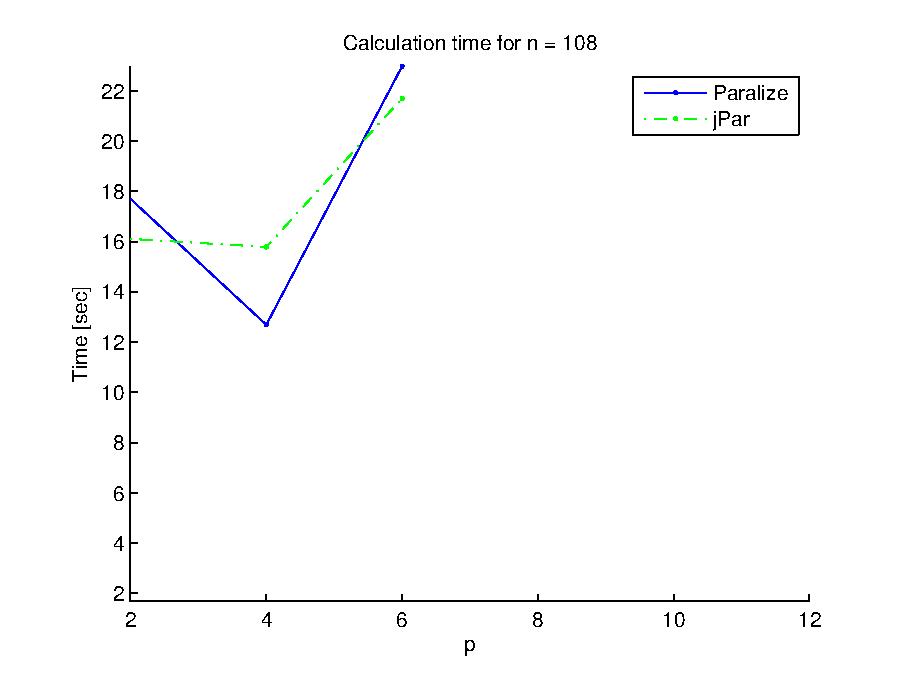
\includegraphics[height=6.5cm]{fig1}
\end{frame}
\begin{frame}
   \frametitle{The speed-up of parallelization and \textcolor{red}{decomposition}}
   \centering
   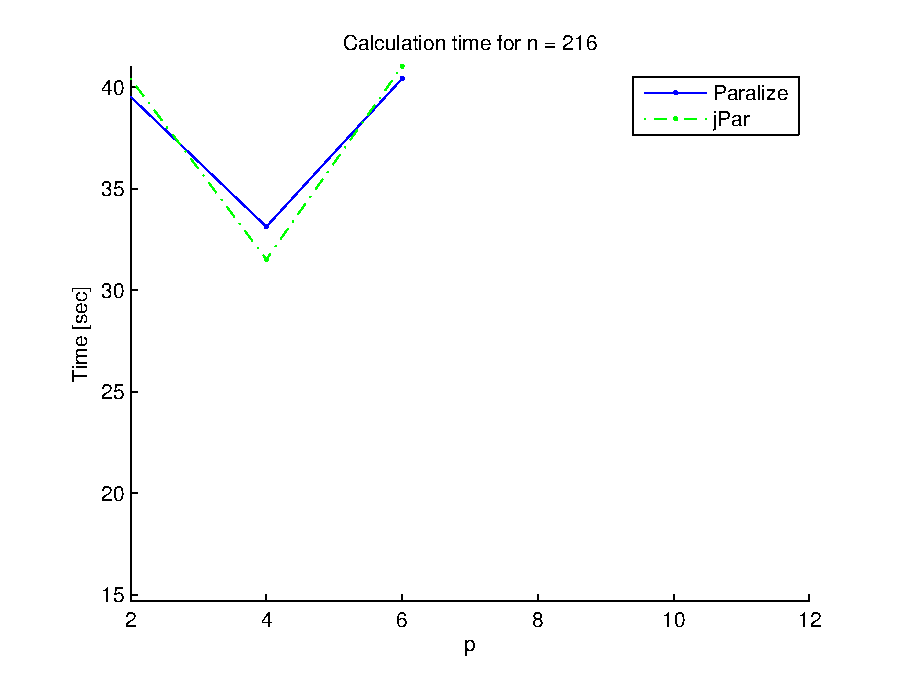
\includegraphics[height=6.5cm]{fig2}
\end{frame}
\begin{frame}
   \frametitle{The speed-up of parallelization and \textcolor{red}{decomposition}}
   \centering
   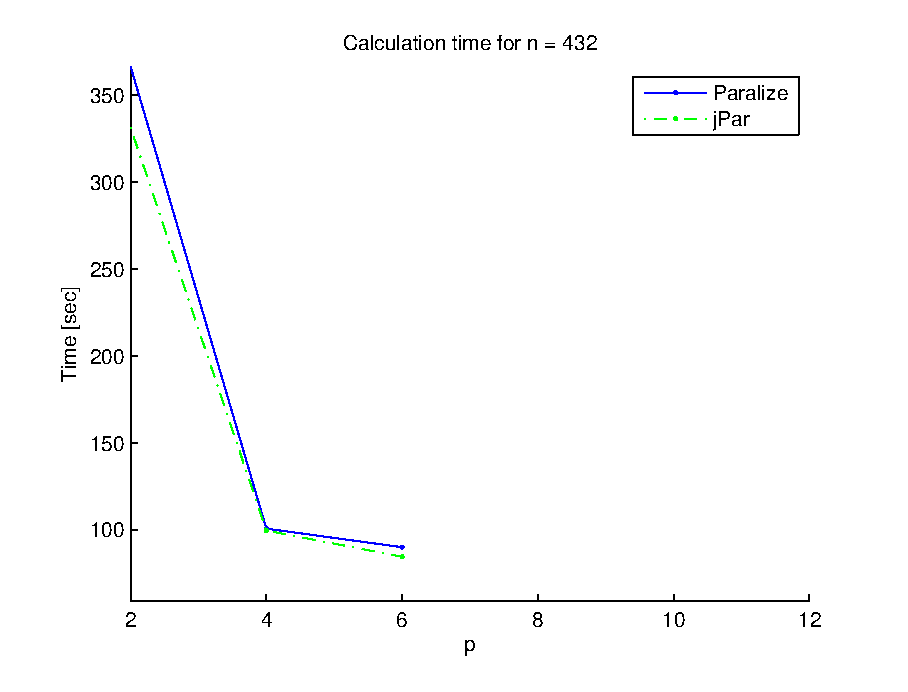
\includegraphics[height=6.5cm]{fig3}
\end{frame}
\begin{frame}
   \frametitle{The speed-up of parallelization and \textcolor{red}{decomposition}}
   \centering
   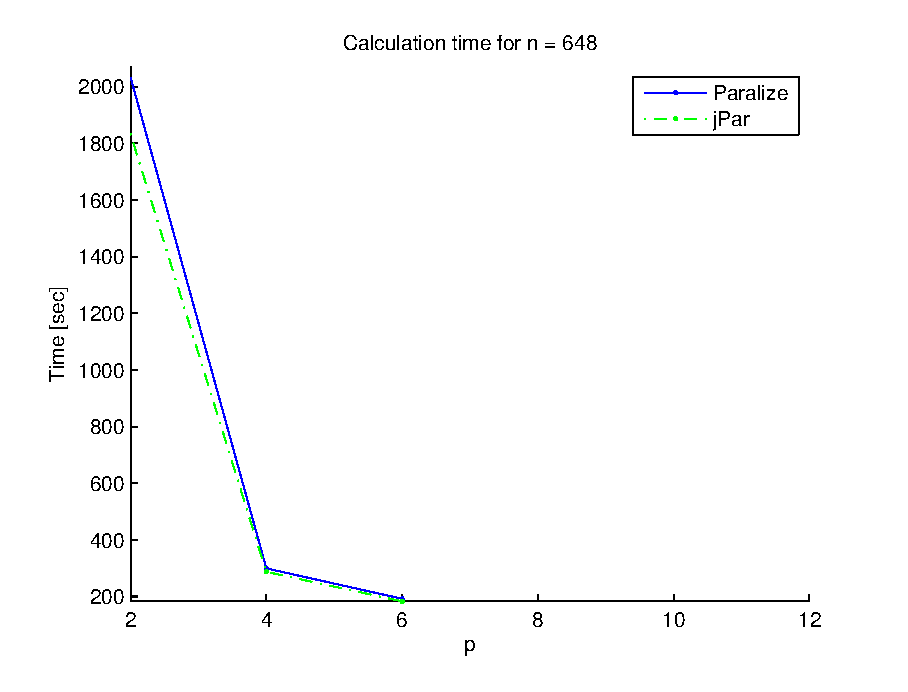
\includegraphics[height=6.5cm]{fig4}
\end{frame}
\begin{frame}
   \frametitle{The speed-up of parallelization and \textcolor{red}{decomposition}}
   \centering
   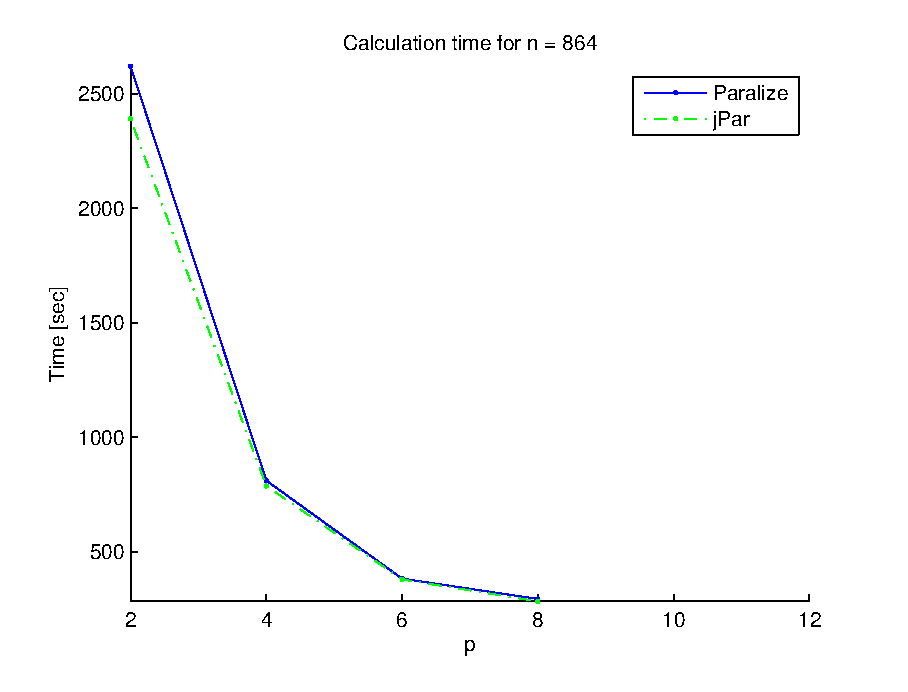
\includegraphics[height=6.5cm]{fig5}
\end{frame}

\section{Plan przyszłych prac}

\begin{frame}[allowframebreaks,fragile]
   \frametitle{Conclusions}
   \begin{enumerate}
      \item The jPar is:
            \begin{itemize}
               \item relatively small (about 800 lines of Java code and 400 lines of Matlab code)
               \item simple in installation
               \item simple in use (the changes in sequential code are very small)
               \item reliable (there are no errors caused by disk transmissions)
               \item heterogenous (Linux, Windows, OS X)
               \item interoperable between various Matlab and Java versions
               \item open and free (can be downloaded from the MatlabCentral page
                     \url{http://www.mathworks.com/matlabcentral/fileexchange/50797} )
            \end{itemize}
            \newpage
      \item Avoiding active
            polling it does not waste the energy, network resources and does
            not block the cores waiting for tasks
      \item The problems that may be solved should have fork-join structure, without communication between instances)
   \end{enumerate}
\end{frame}
\begin{frame}
   \frametitle{Successful application of jPar abroad}
   A beta version of {\emph jPar}  in:
   \begin{enumerate}
      \item MEIGO system: \\
            {\em J.A. Egea, D. Henriques, T. Cokelaer, A.F. Villaverde, A. MacNamara, D.-P. Danciu, J.R. Banga and J. Saez-Rodriguez, ``MEIGO: an open-source software suite based on metaheuristics for global optimization in systems biology and bioinformatics", BMC Bioinformatics, vol. 15,  2014.}
      \item CeSS system:\\
            {\em D.R. Penasa, P. Gonz\'{a}lez , J.A. Egea, J.R. Banga and R. Doallo,
            ``Parallel Metaheuristics in Computational Biology: An Asynchronous Cooperative Enhanced Scatter Search Method", Procedia Computer Science, vol. 51, 2015, pp.  630--639}
   \end{enumerate}
   in Department of Applied Mathematics and Statistics, Universidad Politécnica de Cartagena,
   (Bio)Process Engineering Group, Spanish National Research Council,
   European Molecular Biology Laboratory, Cambridge,
   Instituto de Investigaciones Marinas
\end{frame}
\end{document}
